\documentclass{whiteboard}
\begin{document}
\begin{frame}[plain,t]
\bbcover{Programação Lógica}{Lógica Proposicional Booleana}{Prof. Edson Alves}{Campus UnB Gama: Faculdade de Ciências e Tecnologias em Engenharia}

\end{frame}
\begin{frame}[plain,t]
\begin{tikzpicture}
\node[draw,opacity=0] at (0, 0) {x};
\node[draw,opacity=0] at (14, 8) {x};

	\node[anchor=west] (title) at (0.0, 7.0) { \Large \bbbold{George Boole} };

	\node[] (moses) at (3.0, 4.0) { \includegraphics[scale=0.2]{figs/george-boole.png} };

	\node[anchor=west] (flag) at (1.2, 1.2) { \includegraphics[scale=0.005]{figs/england.png} };

	\node[] (dates) at (3.5, 1.2) { * \bbtext{1815} \hspace*{0.05in} \bbtext{\textdagger\ 1864} };

\end{tikzpicture}
\end{frame}
\begin{frame}[plain,t]
\begin{tikzpicture}
\node[draw,opacity=0] at (0, 0) {x};
\node[draw,opacity=0] at (14, 8) {x};

	\node[anchor=west] (title) at (0.0, 7.0) { \Large \bbbold{George Boole} };

	\node[] (moses) at (3.0, 4.0) { \includegraphics[scale=0.2]{figs/george-boole.png} };

	\node[anchor=west] (flag) at (1.2, 1.2) { \includegraphics[scale=0.005]{figs/england.png} };

	\node[] (dates) at (3.5, 1.2) { * \bbtext{1815} \hspace*{0.05in} \bbtext{\textdagger\ 1864} };


	\node[anchor=west] (article) at (6.0, 6.0) { \large {\bbnote{The Mathematic Analysis of Logic (1847)}} };

\end{tikzpicture}
\end{frame}
\begin{frame}[plain,t]
\begin{tikzpicture}
\node[draw,opacity=0] at (0, 0) {x};
\node[draw,opacity=0] at (14, 8) {x};

	\node[anchor=west] (title) at (0.0, 7.0) { \Large \bbbold{George Boole} };

	\node[] (moses) at (3.0, 4.0) { \includegraphics[scale=0.2]{figs/george-boole.png} };

	\node[anchor=west] (flag) at (1.2, 1.2) { \includegraphics[scale=0.005]{figs/england.png} };

	\node[] (dates) at (3.5, 1.2) { * \bbtext{1815} \hspace*{0.05in} \bbtext{\textdagger\ 1864} };


	\node[anchor=west] (article) at (6.0, 6.0) { \large {\bbnote{The Mathematic Analysis of Logic (1847)}} };


	\node[anchor=west] (a) at (6.5, 5.0) { $\star$ \bbtext{Proposta de formalização da lógica por meio da} };

	\node[anchor=west] (b) at (6.0, 4.5) { \bbtext{matemática} };

\end{tikzpicture}
\end{frame}
\begin{frame}[plain,t]
\begin{tikzpicture}
\node[draw,opacity=0] at (0, 0) {x};
\node[draw,opacity=0] at (14, 8) {x};

	\node[anchor=west] (title) at (0.0, 7.0) { \Large \bbbold{George Boole} };

	\node[] (moses) at (3.0, 4.0) { \includegraphics[scale=0.2]{figs/george-boole.png} };

	\node[anchor=west] (flag) at (1.2, 1.2) { \includegraphics[scale=0.005]{figs/england.png} };

	\node[] (dates) at (3.5, 1.2) { * \bbtext{1815} \hspace*{0.05in} \bbtext{\textdagger\ 1864} };


	\node[anchor=west] (article) at (6.0, 6.0) { \large {\bbnote{The Mathematic Analysis of Logic (1847)}} };


	\node[anchor=west] (a) at (6.5, 5.0) { $\star$ \bbtext{Proposta de formalização da lógica por meio da} };

	\node[anchor=west] (b) at (6.0, 4.5) { \bbtext{matemática} };


	\node[anchor=west] (c) at (6.5, 3.5) { $\star$ \bbtext{O livro introduz os fundamentos da lógica} };

	\node[anchor=west] (c1) at (6.0, 3.0) { \bbtext{proposicional booleana} };

\end{tikzpicture}
\end{frame}
\begin{frame}[plain,t]
\begin{tikzpicture}
\node[draw,opacity=0] at (0, 0) {x};
\node[draw,opacity=0] at (14, 8) {x};

	\node[anchor=west] (title) at (0.0, 7.0) { \Large \bbbold{George Boole} };

	\node[] (moses) at (3.0, 4.0) { \includegraphics[scale=0.2]{figs/george-boole.png} };

	\node[anchor=west] (flag) at (1.2, 1.2) { \includegraphics[scale=0.005]{figs/england.png} };

	\node[] (dates) at (3.5, 1.2) { * \bbtext{1815} \hspace*{0.05in} \bbtext{\textdagger\ 1864} };


	\node[anchor=west] (article) at (6.0, 6.0) { \large {\bbnote{The Mathematic Analysis of Logic (1847)}} };


	\node[anchor=west] (a) at (6.5, 5.0) { $\star$ \bbtext{Proposta de formalização da lógica por meio da} };

	\node[anchor=west] (b) at (6.0, 4.5) { \bbtext{matemática} };


	\node[anchor=west] (c) at (6.5, 3.5) { $\star$ \bbtext{O livro introduz os fundamentos da lógica} };

	\node[anchor=west] (c1) at (6.0, 3.0) { \bbtext{proposicional booleana} };


	\node[anchor=west] (d) at (6.5, 2.0) { $\star$ \bbtext{Ele resgata e expande estes fundamentos no seu} };

	\node[anchor=west] (d1) at (6.0, 1.5) { \bbtext{livro mais conhecido, } \bbnote{An Investigation of the Laws} };

	\node[anchor=west] (d2) at (6.0, 1.0) { \bbnote{of Thought (1849)} };

\end{tikzpicture}
\end{frame}
\begin{frame}[plain,t]
\begin{tikzpicture}
\node[draw,opacity=0] at (0, 0) {x};
\node[draw,opacity=0] at (14, 8) {x};

	\node[anchor=west] (title) at (0.0, 7.0) { \Large \bbbold{Lógica Proposicional Booleana} };

\end{tikzpicture}
\end{frame}
\begin{frame}[plain,t]
\begin{tikzpicture}
\node[draw,opacity=0] at (0, 0) {x};
\node[draw,opacity=0] at (14, 8) {x};

	\node[anchor=west] (title) at (0.0, 7.0) { \Large \bbbold{Lógica Proposicional Booleana} };


	\node[anchor=west] (terms) at (0.5, 5.0) { \bbemph{Termos primitivos} };

\end{tikzpicture}
\end{frame}
\begin{frame}[plain,t]
\begin{tikzpicture}
\node[draw,opacity=0] at (0, 0) {x};
\node[draw,opacity=0] at (14, 8) {x};

	\node[anchor=west] (title) at (0.0, 7.0) { \Large \bbbold{Lógica Proposicional Booleana} };


	\node[anchor=west] (terms) at (0.5, 5.0) { \bbemph{Termos primitivos} };


	\node[anchor=west] (a) at (1.0, 4.0) { $\star$ \bbtext{Proposição} };

\end{tikzpicture}
\end{frame}
\begin{frame}[plain,t]
\begin{tikzpicture}
\node[draw,opacity=0] at (0, 0) {x};
\node[draw,opacity=0] at (14, 8) {x};

	\node[anchor=west] (title) at (0.0, 7.0) { \Large \bbbold{Lógica Proposicional Booleana} };


	\node[anchor=west] (terms) at (0.5, 5.0) { \bbemph{Termos primitivos} };


	\node[anchor=west] (a) at (1.0, 4.0) { $\star$ \bbtext{Proposição} };


	\node[anchor=west] (b) at (1.0, 3.0) { $\star$ \bbtext{Verdadeiro} };

\end{tikzpicture}
\end{frame}
\begin{frame}[plain,t]
\begin{tikzpicture}
\node[draw,opacity=0] at (0, 0) {x};
\node[draw,opacity=0] at (14, 8) {x};

	\node[anchor=west] (title) at (0.0, 7.0) { \Large \bbbold{Lógica Proposicional Booleana} };


	\node[anchor=west] (terms) at (0.5, 5.0) { \bbemph{Termos primitivos} };


	\node[anchor=west] (a) at (1.0, 4.0) { $\star$ \bbtext{Proposição} };


	\node[anchor=west] (b) at (1.0, 3.0) { $\star$ \bbtext{Verdadeiro} };


	\node[anchor=west] (c) at (1.0, 2.0) { $\star$ \bbtext{Falso} };


\end{tikzpicture}
\end{frame}
\begin{frame}[plain,t]
\begin{tikzpicture}
\node[draw,opacity=0] at (0, 0) {x};
\node[draw,opacity=0] at (14, 8) {x};

	\node[anchor=west] (title) at (0.0, 7.0) { \Large \bbbold{Lógica Proposicional Booleana} };


	\node[anchor=west] (terms) at (0.5, 5.0) { \bbemph{Termos primitivos} };


	\node[anchor=west] (a) at (1.0, 4.0) { $\star$ \bbtext{Proposição} };


	\node[anchor=west] (b) at (1.0, 3.0) { $\star$ \bbtext{Verdadeiro} };


	\node[anchor=west] (c) at (1.0, 2.0) { $\star$ \bbtext{Falso} };



	\node[anchor=west] (axioms) at (7.0, 5.0) { \bbemph{Axiomas} };

\end{tikzpicture}
\end{frame}
\begin{frame}[plain,t]
\begin{tikzpicture}
\node[draw,opacity=0] at (0, 0) {x};
\node[draw,opacity=0] at (14, 8) {x};

	\node[anchor=west] (title) at (0.0, 7.0) { \Large \bbbold{Lógica Proposicional Booleana} };


	\node[anchor=west] (terms) at (0.5, 5.0) { \bbemph{Termos primitivos} };


	\node[anchor=west] (a) at (1.0, 4.0) { $\star$ \bbtext{Proposição} };


	\node[anchor=west] (b) at (1.0, 3.0) { $\star$ \bbtext{Verdadeiro} };


	\node[anchor=west] (c) at (1.0, 2.0) { $\star$ \bbtext{Falso} };



	\node[anchor=west] (axioms) at (7.0, 5.0) { \bbemph{Axiomas} };


	\node[anchor=west] (d) at (7.5, 4.0) { $\star$ \bbtext{Princípio do terceiro excluído} };

\end{tikzpicture}
\end{frame}
\begin{frame}[plain,t]
\begin{tikzpicture}
\node[draw,opacity=0] at (0, 0) {x};
\node[draw,opacity=0] at (14, 8) {x};

	\node[anchor=west] (title) at (0.0, 7.0) { \Large \bbbold{Lógica Proposicional Booleana} };


	\node[anchor=west] (terms) at (0.5, 5.0) { \bbemph{Termos primitivos} };


	\node[anchor=west] (a) at (1.0, 4.0) { $\star$ \bbtext{Proposição} };


	\node[anchor=west] (b) at (1.0, 3.0) { $\star$ \bbtext{Verdadeiro} };


	\node[anchor=west] (c) at (1.0, 2.0) { $\star$ \bbtext{Falso} };



	\node[anchor=west] (axioms) at (7.0, 5.0) { \bbemph{Axiomas} };


	\node[anchor=west] (d) at (7.5, 4.0) { $\star$ \bbtext{Princípio do terceiro excluído} };


	\node[anchor=west] (e) at (7.5, 3.0) { $\star$ \bbtext{Princípio da não-contradição} };

\end{tikzpicture}
\end{frame}
\begin{frame}[plain,t]
\begin{tikzpicture}
\node[draw,opacity=0] at (0, 0) {x};
\node[draw,opacity=0] at (14, 8) {x};

	\node[anchor=west] (title) at (0.0, 7.0) { \Large \bbbold{Prolog (1972)} };

\end{tikzpicture}
\end{frame}
\begin{frame}[plain,t]
\begin{tikzpicture}
\node[draw,opacity=0] at (0, 0) {x};
\node[draw,opacity=0] at (14, 8) {x};

	\node[anchor=west] (title) at (0.0, 7.0) { \Large \bbbold{Prolog (1972)} };


	\node[] (a) at (4.0, 6.0) { \bbemph{Proponentes} };

\end{tikzpicture}
\end{frame}
\begin{frame}[plain,t]
\begin{tikzpicture}
\node[draw,opacity=0] at (0, 0) {x};
\node[draw,opacity=0] at (14, 8) {x};

	\node[anchor=west] (title) at (0.0, 7.0) { \Large \bbbold{Prolog (1972)} };


	\node[] (a) at (4.0, 6.0) { \bbemph{Proponentes} };


	\node[] (alain) at (2.0, 3.0) { \includegraphics[scale=0.35]{figs/alain.jpg} };

	\node[] (alain_name) at (2.0, 0.5) { \bbtext{Alain Colmerauer} };

\end{tikzpicture}
\end{frame}
\begin{frame}[plain,t]
\begin{tikzpicture}
\node[draw,opacity=0] at (0, 0) {x};
\node[draw,opacity=0] at (14, 8) {x};

	\node[anchor=west] (title) at (0.0, 7.0) { \Large \bbbold{Prolog (1972)} };


	\node[] (a) at (4.0, 6.0) { \bbemph{Proponentes} };


	\node[] (alain) at (2.0, 3.0) { \includegraphics[scale=0.35]{figs/alain.jpg} };

	\node[] (alain_name) at (2.0, 0.5) { \bbtext{Alain Colmerauer} };


	\node[] (philippe) at (6.5, 3.0) { \includegraphics[scale=0.4]{figs/philippe.jpg} };

	\node[] (philippe_name) at (6.5, 0.5) { \bbtext{Philippe Roussel} };

\end{tikzpicture}
\end{frame}
\begin{frame}[plain,t]
\begin{tikzpicture}
\node[draw,opacity=0] at (0, 0) {x};
\node[draw,opacity=0] at (14, 8) {x};

	\node[anchor=west] (title) at (0.0, 7.0) { \Large \bbbold{Prolog (1972)} };


	\node[] (a) at (4.0, 6.0) { \bbemph{Proponentes} };


	\node[] (alain) at (2.0, 3.0) { \includegraphics[scale=0.35]{figs/alain.jpg} };

	\node[] (alain_name) at (2.0, 0.5) { \bbtext{Alain Colmerauer} };


	\node[] (philippe) at (6.5, 3.0) { \includegraphics[scale=0.4]{figs/philippe.jpg} };

	\node[] (philippe_name) at (6.5, 0.5) { \bbtext{Philippe Roussel} };


	\node[] (b) at (11.0, 6.0) { \bbemph{Inspiração} };

\end{tikzpicture}
\end{frame}
\begin{frame}[plain,t]
\begin{tikzpicture}
\node[draw,opacity=0] at (0, 0) {x};
\node[draw,opacity=0] at (14, 8) {x};

	\node[anchor=west] (title) at (0.0, 7.0) { \Large \bbbold{Prolog (1972)} };


	\node[] (a) at (4.0, 6.0) { \bbemph{Proponentes} };


	\node[] (alain) at (2.0, 3.0) { \includegraphics[scale=0.35]{figs/alain.jpg} };

	\node[] (alain_name) at (2.0, 0.5) { \bbtext{Alain Colmerauer} };


	\node[] (philippe) at (6.5, 3.0) { \includegraphics[scale=0.4]{figs/philippe.jpg} };

	\node[] (philippe_name) at (6.5, 0.5) { \bbtext{Philippe Roussel} };


	\node[] (b) at (11.0, 6.0) { \bbemph{Inspiração} };


	\node[] (robert) at (11.0, 3.0) { \includegraphics[scale=0.35]{figs/robert.jpg} };

	\node[] (robert_name) at (11.0, 0.5) { \bbtext{Robert Kowalski} };

\end{tikzpicture}
\end{frame}
\begin{frame}[plain,t]
\begin{tikzpicture}
\node[draw,opacity=0] at (0, 0) {x};
\node[draw,opacity=0] at (14, 8) {x};

	\node[anchor=west] (title) at (0.0, 7.0) { \Large \bbbold{SWI Prolog} };

\end{tikzpicture}
\end{frame}
\begin{frame}[plain,t]
\begin{tikzpicture}
\node[draw,opacity=0] at (0, 0) {x};
\node[draw,opacity=0] at (14, 8) {x};

	\node[anchor=west] (title) at (0.0, 7.0) { \Large \bbbold{SWI Prolog} };


	\node[anchor=west] (a) at (1.0, 6.0) { $\star$ \bbtext{ Prolog é uma contração da expressão ``PROgramming in LOGic''} };

\end{tikzpicture}
\end{frame}
\begin{frame}[plain,t]
\begin{tikzpicture}
\node[draw,opacity=0] at (0, 0) {x};
\node[draw,opacity=0] at (14, 8) {x};

	\node[anchor=west] (title) at (0.0, 7.0) { \Large \bbbold{SWI Prolog} };


	\node[anchor=west] (a) at (1.0, 6.0) { $\star$ \bbtext{ Prolog é uma contração da expressão ``PROgramming in LOGic''} };


	\node[anchor=west] (b) at (1.0, 5.0) { $\star$ \bbtext{Tem raízes na lógica de primeira ordem} };

\end{tikzpicture}
\end{frame}
\begin{frame}[plain,t]
\begin{tikzpicture}
\node[draw,opacity=0] at (0, 0) {x};
\node[draw,opacity=0] at (14, 8) {x};

	\node[anchor=west] (title) at (0.0, 7.0) { \Large \bbbold{SWI Prolog} };


	\node[anchor=west] (a) at (1.0, 6.0) { $\star$ \bbtext{ Prolog é uma contração da expressão ``PROgramming in LOGic''} };


	\node[anchor=west] (b) at (1.0, 5.0) { $\star$ \bbtext{Tem raízes na lógica de primeira ordem} };


	\node[anchor=west] (c1) at (1.0, 4.0) { $\star$ \bbtext{O SWI-Prolog pode ser instalado por meio do comando} };

	\node[anchor=west] (c2) at (2.0, 3.0) { \mintinline{bash}{$ sudo apt-get install swi-prolog} };

\end{tikzpicture}
\end{frame}
\begin{frame}[plain,t]
\begin{tikzpicture}
\node[draw,opacity=0] at (0, 0) {x};
\node[draw,opacity=0] at (14, 8) {x};

	\node[anchor=west] (title) at (0.0, 7.0) { \Large \bbbold{SWI Prolog} };


	\node[anchor=west] (a) at (1.0, 6.0) { $\star$ \bbtext{ Prolog é uma contração da expressão ``PROgramming in LOGic''} };


	\node[anchor=west] (b) at (1.0, 5.0) { $\star$ \bbtext{Tem raízes na lógica de primeira ordem} };


	\node[anchor=west] (c1) at (1.0, 4.0) { $\star$ \bbtext{O SWI-Prolog pode ser instalado por meio do comando} };

	\node[anchor=west] (c2) at (2.0, 3.0) { \mintinline{bash}{$ sudo apt-get install swi-prolog} };


	\node[anchor=west] (d1) at (1.0, 2.0) { $\star$ \bbtext{O interpretador (}\bbenglish{listener}\bbtext{) Prolog pode ser invocado com o comando} };

	\node[anchor=west] (d2) at (2.0, 1.0) { \mintinline{bash}{$ prolog} };

\end{tikzpicture}
\end{frame}
\begin{frame}[plain,t]
\begin{tikzpicture}
\node[draw,opacity=0] at (0, 0) {x};
\node[draw,opacity=0] at (14, 8) {x};

	\node[anchor=west] (title) at (0.0, 7.0) { \Large \bbbold{Valores lógicos em Prolog} };

\end{tikzpicture}
\end{frame}
\begin{frame}[plain,t]
\begin{tikzpicture}
\node[draw,opacity=0] at (0, 0) {x};
\node[draw,opacity=0] at (14, 8) {x};

	\node[anchor=west] (title) at (0.0, 7.0) { \Large \bbbold{Valores lógicos em Prolog} };


	\node[anchor=west] (a1) at (1.0, 6.0) { $\star$ \bbtext{Prolog implementa os termos primitivos} \bbenglish{verdadeiro} \bbtext{e} \bbenglish{falso} \bbtext{por meio dos} };

	\node[anchor=west] (a2) at (0.5, 5.5) { \bbtext{predicados \code{prolog}{true/0} e \code{prolog}{false/0}} };

\end{tikzpicture}
\end{frame}
\begin{frame}[plain,t]
\begin{tikzpicture}
\node[draw,opacity=0] at (0, 0) {x};
\node[draw,opacity=0] at (14, 8) {x};

	\node[anchor=west] (title) at (0.0, 7.0) { \Large \bbbold{Valores lógicos em Prolog} };


	\node[anchor=west] (a1) at (1.0, 6.0) { $\star$ \bbtext{Prolog implementa os termos primitivos} \bbenglish{verdadeiro} \bbtext{e} \bbenglish{falso} \bbtext{por meio dos} };

	\node[anchor=west] (a2) at (0.5, 5.5) { \bbtext{predicados \code{prolog}{true/0} e \code{prolog}{false/0}} };


	\node[anchor=west] (b) at (2.0, 4.0) { \inputsyntax{prolog}{codes/true_false.pl} };

\end{tikzpicture}
\end{frame}
\begin{frame}[plain,t]
\begin{tikzpicture}
\node[draw,opacity=0] at (0, 0) {x};
\node[draw,opacity=0] at (14, 8) {x};

	\node[anchor=west] (title) at (0.0, 7.0) { \Large \bbbold{Valores lógicos em Prolog} };


	\node[anchor=west] (a1) at (1.0, 6.0) { $\star$ \bbtext{Prolog implementa os termos primitivos} \bbenglish{verdadeiro} \bbtext{e} \bbenglish{falso} \bbtext{por meio dos} };

	\node[anchor=west] (a2) at (0.5, 5.5) { \bbtext{predicados \code{prolog}{true/0} e \code{prolog}{false/0}} };


	\node[anchor=west] (b) at (2.0, 4.0) { \inputsyntax{prolog}{codes/true_false.pl} };


	\node[anchor=west] (c) at (1.0, 2.5) { $\star$ \bbtext{Prolog faz distinção entre maiúsculas e minúsculas} };


\end{tikzpicture}
\end{frame}
\begin{frame}[plain,t]
\begin{tikzpicture}
\node[draw,opacity=0] at (0, 0) {x};
\node[draw,opacity=0] at (14, 8) {x};

	\node[anchor=west] (title) at (0.0, 7.0) { \Large \bbbold{Valores lógicos em Prolog} };


	\node[anchor=west] (a1) at (1.0, 6.0) { $\star$ \bbtext{Prolog implementa os termos primitivos} \bbenglish{verdadeiro} \bbtext{e} \bbenglish{falso} \bbtext{por meio dos} };

	\node[anchor=west] (a2) at (0.5, 5.5) { \bbtext{predicados \code{prolog}{true/0} e \code{prolog}{false/0}} };


	\node[anchor=west] (b) at (2.0, 4.0) { \inputsyntax{prolog}{codes/true_false.pl} };


	\node[anchor=west] (c) at (1.0, 2.5) { $\star$ \bbtext{Prolog faz distinção entre maiúsculas e minúsculas} };



	\node[anchor=west] (d) at (2.0, 1.25) { \inputsyntax{prolog}{codes/42.pl} };

\end{tikzpicture}
\end{frame}
\begin{frame}[plain,t]
\begin{tikzpicture}
\node[draw,opacity=0] at (0, 0) {x};
\node[draw,opacity=0] at (14, 8) {x};

	\node[anchor=west] (title) at (0.0, 7.0) { \Large \bbbold{Conectivos da lógica proposicional booleana} };

\end{tikzpicture}
\end{frame}
\begin{frame}[plain,t]
\begin{tikzpicture}
\node[draw,opacity=0] at (0, 0) {x};
\node[draw,opacity=0] at (14, 8) {x};

	\node[anchor=west] (title) at (0.0, 7.0) { \Large \bbbold{Conectivos da lógica proposicional booleana} };


	\draw[very thick] (0.0, 6.0) to  (13.0, 6.0);

	\draw[thick] (0.0, 5.0) to  (13.0, 5.0);

	\node[anchor=west] (op) at (0.25, 5.5) { \bbemph{Operação} };

	\node[anchor=west] (read) at (3.0, 5.5) { \bbemph{Leitura} };

	\node[anchor=west] (desc) at (5.5, 5.5) { \bbemph{Definição} };

\end{tikzpicture}
\end{frame}
\begin{frame}[plain,t]
\begin{tikzpicture}
\node[draw,opacity=0] at (0, 0) {x};
\node[draw,opacity=0] at (14, 8) {x};

	\node[anchor=west] (title) at (0.0, 7.0) { \Large \bbbold{Conectivos da lógica proposicional booleana} };


	\draw[very thick] (0.0, 6.0) to  (13.0, 6.0);

	\draw[thick] (0.0, 5.0) to  (13.0, 5.0);

	\node[anchor=west] (op) at (0.25, 5.5) { \bbemph{Operação} };

	\node[anchor=west] (read) at (3.0, 5.5) { \bbemph{Leitura} };

	\node[anchor=west] (desc) at (5.5, 5.5) { \bbemph{Definição} };


	\node[] (not) at (1.2, 4.5) { $\lnot a$ };

	\node[] (not_read) at (3.8, 4.5) { \footnotesize \bbtext{não $a$} };

	\node[anchor=west] (not_desc) at (5.5, 4.5) { \footnotesize \bbtext{Inverte o valor lógico de $a$} };

\end{tikzpicture}
\end{frame}
\begin{frame}[plain,t]
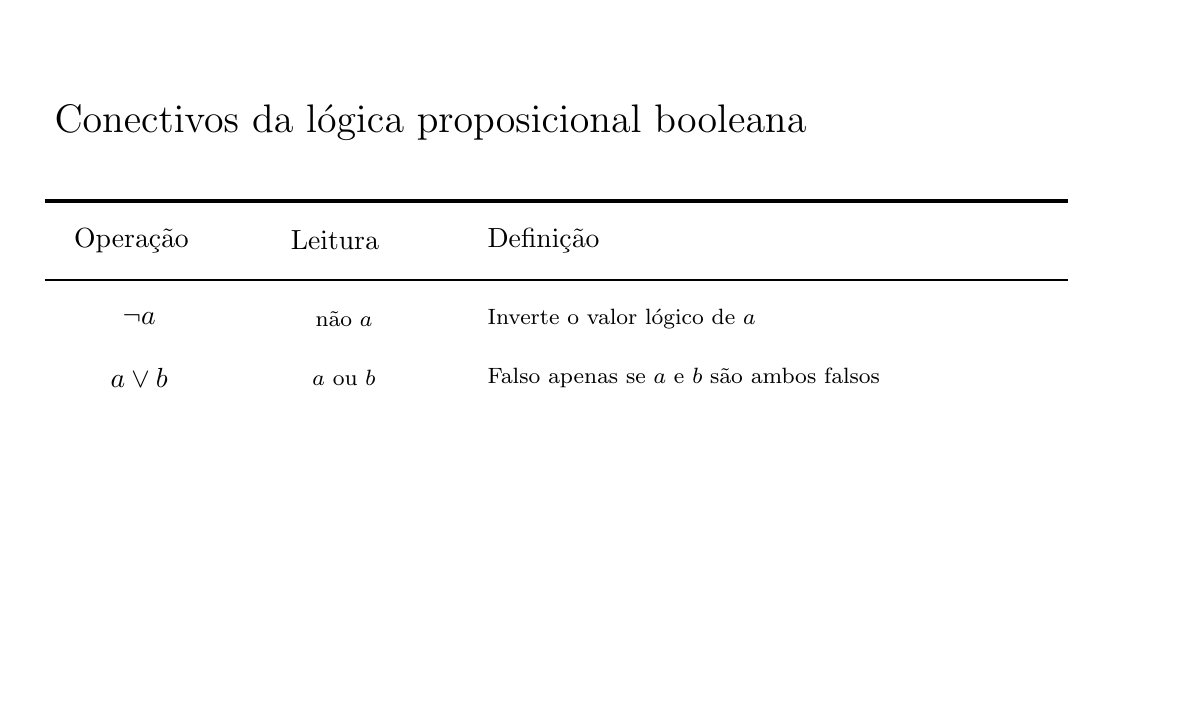
\begin{tikzpicture}
\node[draw,opacity=0] at (0, 0) {x};
\node[draw,opacity=0] at (14, 8) {x};

	\node[anchor=west] (title) at (0.0, 7.0) { \Large \bbbold{Conectivos da lógica proposicional booleana} };


	\draw[very thick] (0.0, 6.0) to  (13.0, 6.0);

	\draw[thick] (0.0, 5.0) to  (13.0, 5.0);

	\node[anchor=west] (op) at (0.25, 5.5) { \bbemph{Operação} };

	\node[anchor=west] (read) at (3.0, 5.5) { \bbemph{Leitura} };

	\node[anchor=west] (desc) at (5.5, 5.5) { \bbemph{Definição} };


	\node[] (not) at (1.2, 4.5) { $\lnot a$ };

	\node[] (not_read) at (3.8, 4.5) { \footnotesize \bbtext{não $a$} };

	\node[anchor=west] (not_desc) at (5.5, 4.5) { \footnotesize \bbtext{Inverte o valor lógico de $a$} };


	\node[] (or) at (1.2, 3.75) { $a\vee b$ };

	\node[] (or_read) at (3.8, 3.75) { \footnotesize \bbtext{$a$ ou $b$} };

	\node[anchor=west] (or_desc) at (5.5, 3.75) { \footnotesize \bbtext{Falso apenas se $a$ e $b$ são ambos falsos} };

\end{tikzpicture}
\end{frame}
\begin{frame}[plain,t]
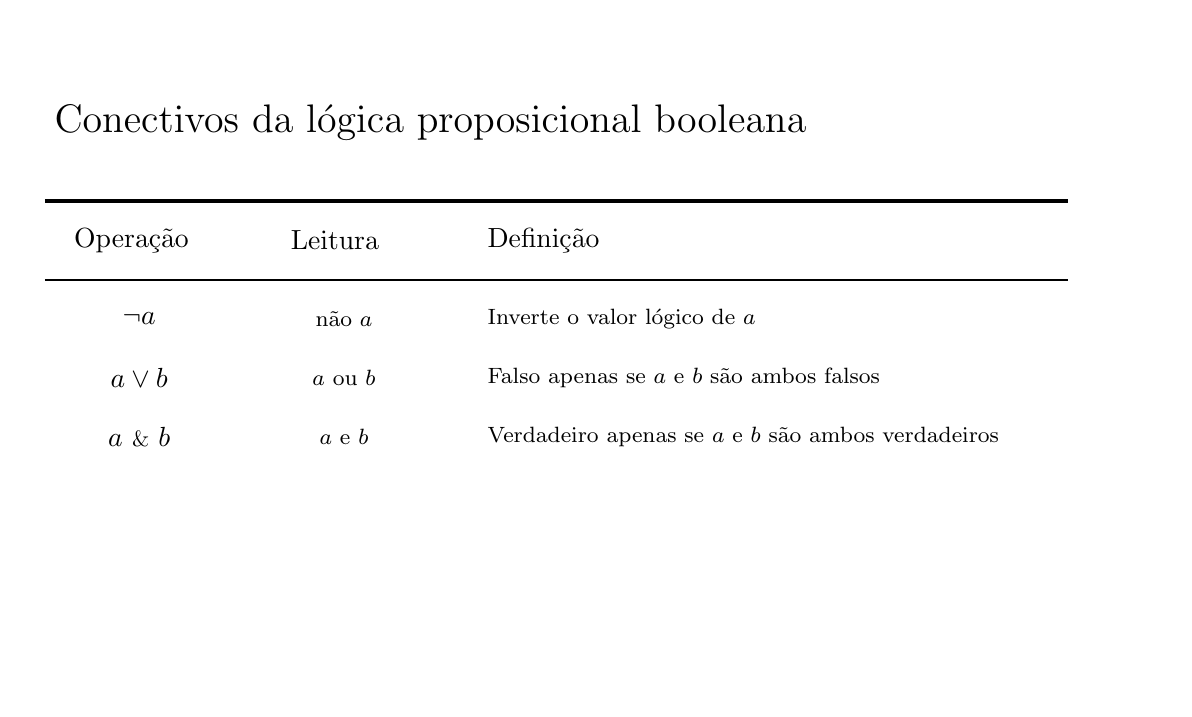
\begin{tikzpicture}
\node[draw,opacity=0] at (0, 0) {x};
\node[draw,opacity=0] at (14, 8) {x};

	\node[anchor=west] (title) at (0.0, 7.0) { \Large \bbbold{Conectivos da lógica proposicional booleana} };


	\draw[very thick] (0.0, 6.0) to  (13.0, 6.0);

	\draw[thick] (0.0, 5.0) to  (13.0, 5.0);

	\node[anchor=west] (op) at (0.25, 5.5) { \bbemph{Operação} };

	\node[anchor=west] (read) at (3.0, 5.5) { \bbemph{Leitura} };

	\node[anchor=west] (desc) at (5.5, 5.5) { \bbemph{Definição} };


	\node[] (not) at (1.2, 4.5) { $\lnot a$ };

	\node[] (not_read) at (3.8, 4.5) { \footnotesize \bbtext{não $a$} };

	\node[anchor=west] (not_desc) at (5.5, 4.5) { \footnotesize \bbtext{Inverte o valor lógico de $a$} };


	\node[] (or) at (1.2, 3.75) { $a\vee b$ };

	\node[] (or_read) at (3.8, 3.75) { \footnotesize \bbtext{$a$ ou $b$} };

	\node[anchor=west] (or_desc) at (5.5, 3.75) { \footnotesize \bbtext{Falso apenas se $a$ e $b$ são ambos falsos} };


	\node[] (and) at (1.2, 3.0) { $a\ \scalebox{0.8}\&\  b$ };

	\node[] (and_read) at (3.8, 3.0) { \footnotesize \bbtext{$a$ e $b$} };

	\node[anchor=west] (and_desc) at (5.5, 3.0) { \footnotesize \bbtext{Verdadeiro apenas se $a$ e $b$ são ambos verdadeiros} };

\end{tikzpicture}
\end{frame}
\begin{frame}[plain,t]
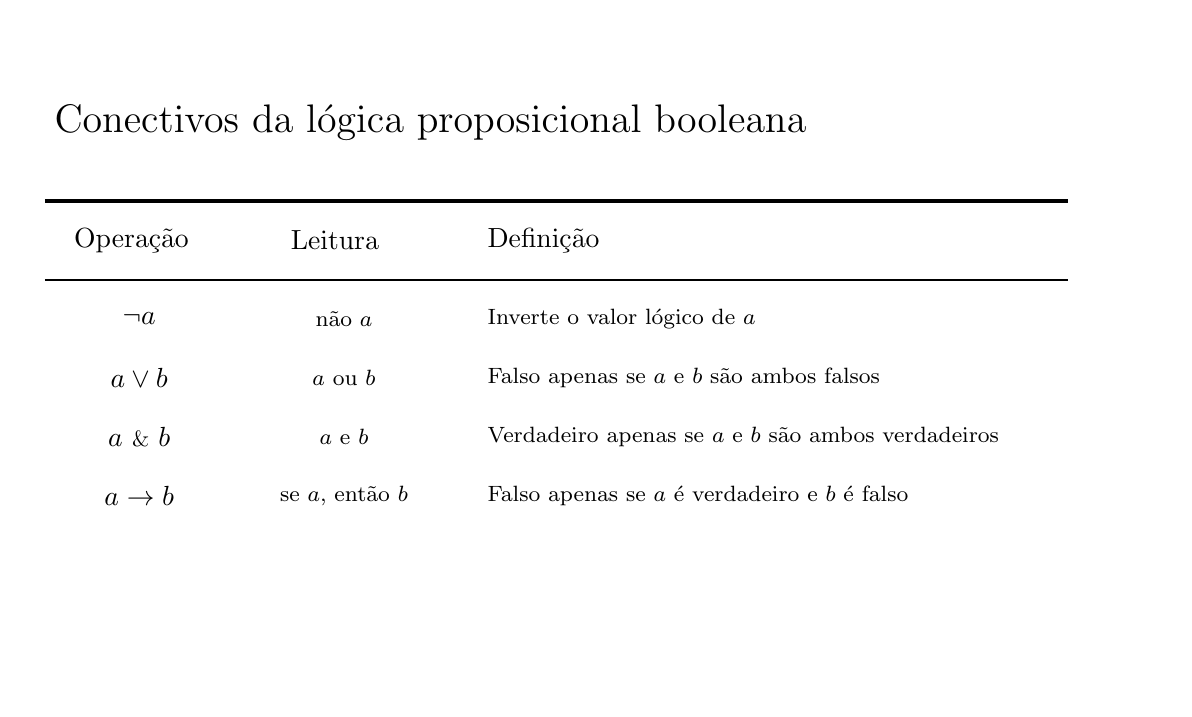
\begin{tikzpicture}
\node[draw,opacity=0] at (0, 0) {x};
\node[draw,opacity=0] at (14, 8) {x};

	\node[anchor=west] (title) at (0.0, 7.0) { \Large \bbbold{Conectivos da lógica proposicional booleana} };


	\draw[very thick] (0.0, 6.0) to  (13.0, 6.0);

	\draw[thick] (0.0, 5.0) to  (13.0, 5.0);

	\node[anchor=west] (op) at (0.25, 5.5) { \bbemph{Operação} };

	\node[anchor=west] (read) at (3.0, 5.5) { \bbemph{Leitura} };

	\node[anchor=west] (desc) at (5.5, 5.5) { \bbemph{Definição} };


	\node[] (not) at (1.2, 4.5) { $\lnot a$ };

	\node[] (not_read) at (3.8, 4.5) { \footnotesize \bbtext{não $a$} };

	\node[anchor=west] (not_desc) at (5.5, 4.5) { \footnotesize \bbtext{Inverte o valor lógico de $a$} };


	\node[] (or) at (1.2, 3.75) { $a\vee b$ };

	\node[] (or_read) at (3.8, 3.75) { \footnotesize \bbtext{$a$ ou $b$} };

	\node[anchor=west] (or_desc) at (5.5, 3.75) { \footnotesize \bbtext{Falso apenas se $a$ e $b$ são ambos falsos} };


	\node[] (and) at (1.2, 3.0) { $a\ \scalebox{0.8}\&\  b$ };

	\node[] (and_read) at (3.8, 3.0) { \footnotesize \bbtext{$a$ e $b$} };

	\node[anchor=west] (and_desc) at (5.5, 3.0) { \footnotesize \bbtext{Verdadeiro apenas se $a$ e $b$ são ambos verdadeiros} };


	\node[] (conditional) at (1.2, 2.25) { $a \to  b$ };

	\node[] (conditional_read) at (3.8, 2.25) { \footnotesize \bbtext{se $a$, então $b$} };

	\node[anchor=west] (conditional_desc) at (5.5, 2.25) { \footnotesize \bbtext{Falso apenas se $a$ é verdadeiro e $b$ é falso} };

\end{tikzpicture}
\end{frame}
\begin{frame}[plain,t]
\begin{tikzpicture}
\node[draw,opacity=0] at (0, 0) {x};
\node[draw,opacity=0] at (14, 8) {x};

	\node[anchor=west] (title) at (0.0, 7.0) { \Large \bbbold{Conectivos da lógica proposicional booleana} };


	\draw[very thick] (0.0, 6.0) to  (13.0, 6.0);

	\draw[thick] (0.0, 5.0) to  (13.0, 5.0);

	\node[anchor=west] (op) at (0.25, 5.5) { \bbemph{Operação} };

	\node[anchor=west] (read) at (3.0, 5.5) { \bbemph{Leitura} };

	\node[anchor=west] (desc) at (5.5, 5.5) { \bbemph{Definição} };


	\node[] (not) at (1.2, 4.5) { $\lnot a$ };

	\node[] (not_read) at (3.8, 4.5) { \footnotesize \bbtext{não $a$} };

	\node[anchor=west] (not_desc) at (5.5, 4.5) { \footnotesize \bbtext{Inverte o valor lógico de $a$} };


	\node[] (or) at (1.2, 3.75) { $a\vee b$ };

	\node[] (or_read) at (3.8, 3.75) { \footnotesize \bbtext{$a$ ou $b$} };

	\node[anchor=west] (or_desc) at (5.5, 3.75) { \footnotesize \bbtext{Falso apenas se $a$ e $b$ são ambos falsos} };


	\node[] (and) at (1.2, 3.0) { $a\ \scalebox{0.8}\&\  b$ };

	\node[] (and_read) at (3.8, 3.0) { \footnotesize \bbtext{$a$ e $b$} };

	\node[anchor=west] (and_desc) at (5.5, 3.0) { \footnotesize \bbtext{Verdadeiro apenas se $a$ e $b$ são ambos verdadeiros} };


	\node[] (conditional) at (1.2, 2.25) { $a \to  b$ };

	\node[] (conditional_read) at (3.8, 2.25) { \footnotesize \bbtext{se $a$, então $b$} };

	\node[anchor=west] (conditional_desc) at (5.5, 2.25) { \footnotesize \bbtext{Falso apenas se $a$ é verdadeiro e $b$ é falso} };


	\node[] (equivalence) at (1.2, 1.5) { $a\ \scalebox{1.2}[0.8]{\leftrightarrow}\ b$ };

	\node[] (equivalence_read) at (3.8, 1.5) { \footnotesize \bbtext{$a$ é equivalente a $b$} };

	\node[anchor=west] (equivalence_desc) at (5.5, 1.5) { \footnotesize \bbtext{Verdadeiro se ambos tem mesmo valor lógico} };


	\draw[very thick] (0.0, 1.0) to  (13.0, 1.0);

\end{tikzpicture}
\end{frame}
\begin{frame}[plain,t]
\begin{tikzpicture}
\node[draw,opacity=0] at (0, 0) {x};
\node[draw,opacity=0] at (14, 8) {x};

	\node[anchor=west] (title) at (0.0, 7.0) { \Large \bbbold{Fatos} };

\end{tikzpicture}
\end{frame}
\begin{frame}[plain,t]
\begin{tikzpicture}
\node[draw,opacity=0] at (0, 0) {x};
\node[draw,opacity=0] at (14, 8) {x};

	\node[anchor=west] (title) at (0.0, 7.0) { \Large \bbbold{Fatos} };

	\node[anchor=west] (a) at (1.0, 6.0) { $\star$ \bbtext{Fatos são os predicados mais simples da linguagem Prolog} };

\end{tikzpicture}
\end{frame}
\begin{frame}[plain,t]
\begin{tikzpicture}
\node[draw,opacity=0] at (0, 0) {x};
\node[draw,opacity=0] at (14, 8) {x};

	\node[anchor=west] (title) at (0.0, 7.0) { \Large \bbbold{Fatos} };

	\node[anchor=west] (a) at (1.0, 6.0) { $\star$ \bbtext{Fatos são os predicados mais simples da linguagem Prolog} };

	\node[anchor=west] (b) at (1.0, 5.0) { $\star$ \bbtext{Eles correspondem a proposições verdadeiras} };

\end{tikzpicture}
\end{frame}
\begin{frame}[plain,t]
\begin{tikzpicture}
\node[draw,opacity=0] at (0, 0) {x};
\node[draw,opacity=0] at (14, 8) {x};

	\node[anchor=west] (title) at (0.0, 7.0) { \Large \bbbold{Fatos} };

	\node[anchor=west] (a) at (1.0, 6.0) { $\star$ \bbtext{Fatos são os predicados mais simples da linguagem Prolog} };

	\node[anchor=west] (b) at (1.0, 5.0) { $\star$ \bbtext{Eles correspondem a proposições verdadeiras} };

	\node[anchor=west] (c) at (1.0, 4.0) { $\star$ \bbtext{A sintaxe para a declaração do fato \code{prolog}{pred/N} é} };

\end{tikzpicture}
\end{frame}
\begin{frame}[plain,t]
\begin{tikzpicture}
\node[draw,opacity=0] at (0, 0) {x};
\node[draw,opacity=0] at (14, 8) {x};

	\node[anchor=west] (title) at (0.0, 7.0) { \Large \bbbold{Fatos} };

	\node[anchor=west] (a) at (1.0, 6.0) { $\star$ \bbtext{Fatos são os predicados mais simples da linguagem Prolog} };

	\node[anchor=west] (b) at (1.0, 5.0) { $\star$ \bbtext{Eles correspondem a proposições verdadeiras} };

	\node[anchor=west] (c) at (1.0, 4.0) { $\star$ \bbtext{A sintaxe para a declaração do fato \code{prolog}{pred/N} é} };

	\node[] (d) at (7.0, 2.5) { \code{prolog}{pred(arg1, arg2, ..., argN).} };

\end{tikzpicture}
\end{frame}
\begin{frame}[plain,t]
\begin{tikzpicture}
\node[draw,opacity=0] at (0, 0) {x};
\node[draw,opacity=0] at (14, 8) {x};

	\node[anchor=west] (title) at (0.0, 7.0) { \Large \bbbold{Fatos} };

	\node[anchor=west] (a) at (1.0, 6.0) { $\star$ \bbtext{Fatos são os predicados mais simples da linguagem Prolog} };

	\node[anchor=west] (b) at (1.0, 5.0) { $\star$ \bbtext{Eles correspondem a proposições verdadeiras} };

	\node[anchor=west] (c) at (1.0, 4.0) { $\star$ \bbtext{A sintaxe para a declaração do fato \code{prolog}{pred/N} é} };

	\node[] (d) at (7.0, 2.5) { \code{prolog}{pred(arg1, arg2, ..., argN).} };


	\node[anchor=east] (d1) at (3.5, 3.25) { \bbcomment{nome} };

	\draw[color=BBViolet,thick] (4.2, 2.8) to  (5.0, 2.8);

	\draw[color=BBViolet,-latex,thick] (4.6, 2.8) -- (4.6, 3.25) -- (3.5, 3.25);

\end{tikzpicture}
\end{frame}
\begin{frame}[plain,t]
\begin{tikzpicture}
\node[draw,opacity=0] at (0, 0) {x};
\node[draw,opacity=0] at (14, 8) {x};

	\node[anchor=west] (title) at (0.0, 7.0) { \Large \bbbold{Fatos} };

	\node[anchor=west] (a) at (1.0, 6.0) { $\star$ \bbtext{Fatos são os predicados mais simples da linguagem Prolog} };

	\node[anchor=west] (b) at (1.0, 5.0) { $\star$ \bbtext{Eles correspondem a proposições verdadeiras} };

	\node[anchor=west] (c) at (1.0, 4.0) { $\star$ \bbtext{A sintaxe para a declaração do fato \code{prolog}{pred/N} é} };

	\node[] (d) at (7.0, 2.5) { \code{prolog}{pred(arg1, arg2, ..., argN).} };


	\node[anchor=east] (d1) at (3.5, 3.25) { \bbcomment{nome} };

	\draw[color=BBViolet,thick] (4.2, 2.8) to  (5.0, 2.8);

	\draw[color=BBViolet,-latex,thick] (4.6, 2.8) -- (4.6, 3.25) -- (3.5, 3.25);


	\node[] (d2) at (7.3, 1.2) { \bbcomment{argumentos} };

	\draw[color=BBViolet,thick] (5.25, 2.3) -- (5.25, 2.2) -- (9.35, 2.2) -- (9.35, 2.3);

	\draw[color=BBViolet,thick,-latex] (7.3, 2.2) to  (7.3, 1.5);


\end{tikzpicture}
\end{frame}
\begin{frame}[plain,t]
\begin{tikzpicture}
\node[draw,opacity=0] at (0, 0) {x};
\node[draw,opacity=0] at (14, 8) {x};

	\node[anchor=west] (title) at (0.0, 7.0) { \Large \bbbold{Fatos} };

	\node[anchor=west] (a) at (1.0, 6.0) { $\star$ \bbtext{Fatos são os predicados mais simples da linguagem Prolog} };

	\node[anchor=west] (b) at (1.0, 5.0) { $\star$ \bbtext{Eles correspondem a proposições verdadeiras} };

	\node[anchor=west] (c) at (1.0, 4.0) { $\star$ \bbtext{A sintaxe para a declaração do fato \code{prolog}{pred/N} é} };

	\node[] (d) at (7.0, 2.5) { \code{prolog}{pred(arg1, arg2, ..., argN).} };


	\node[anchor=east] (d1) at (3.5, 3.25) { \bbcomment{nome} };

	\draw[color=BBViolet,thick] (4.2, 2.8) to  (5.0, 2.8);

	\draw[color=BBViolet,-latex,thick] (4.6, 2.8) -- (4.6, 3.25) -- (3.5, 3.25);


	\node[] (d2) at (7.3, 1.2) { \bbcomment{argumentos} };

	\draw[color=BBViolet,thick] (5.25, 2.3) -- (5.25, 2.2) -- (9.35, 2.2) -- (9.35, 2.3);

	\draw[color=BBViolet,thick,-latex] (7.3, 2.2) to  (7.3, 1.5);



	\node[anchor=west] (d3) at (10.0, 3.2) { \bbcomment{aridade} };

	\draw[color=BBViolet,thick,-latex] (9.25, 2.8) -- (9.25, 3.2) -- (10.05, 3.2);

\end{tikzpicture}
\end{frame}
\begin{frame}[plain,t]
\begin{tikzpicture}
\node[draw,opacity=0] at (0, 0) {x};
\node[draw,opacity=0] at (14, 8) {x};

	\node[anchor=west] (title) at (0.0, 7.0) { \Large \bbbold{Fatos} };

	\node[anchor=west] (a) at (1.0, 6.0) { $\star$ \bbtext{Fatos são os predicados mais simples da linguagem Prolog} };

	\node[anchor=west] (b) at (1.0, 5.0) { $\star$ \bbtext{Eles correspondem a proposições verdadeiras} };

	\node[anchor=west] (c) at (1.0, 4.0) { $\star$ \bbtext{A sintaxe para a declaração do fato \code{prolog}{pred/N} é} };

	\node[] (d) at (7.0, 2.5) { \code{prolog}{pred(arg1, arg2, ..., argN).} };


	\node[anchor=east] (d1) at (3.5, 3.25) { \bbcomment{nome} };

	\draw[color=BBViolet,thick] (4.2, 2.8) to  (5.0, 2.8);

	\draw[color=BBViolet,-latex,thick] (4.6, 2.8) -- (4.6, 3.25) -- (3.5, 3.25);


	\node[] (d2) at (7.3, 1.2) { \bbcomment{argumentos} };

	\draw[color=BBViolet,thick] (5.25, 2.3) -- (5.25, 2.2) -- (9.35, 2.2) -- (9.35, 2.3);

	\draw[color=BBViolet,thick,-latex] (7.3, 2.2) to  (7.3, 1.5);



	\node[anchor=west] (d3) at (10.0, 3.2) { \bbcomment{aridade} };

	\draw[color=BBViolet,thick,-latex] (9.25, 2.8) -- (9.25, 3.2) -- (10.05, 3.2);


	\node[anchor=west] (d4) at (10.5, 2.1) { \bbcomment{terminador} };

	\draw[color=BBViolet,thick,-latex] (9.675, 2.3) -- (9.675, 2.1) -- (10.5, 2.1);

\end{tikzpicture}
\end{frame}
\begin{frame}[plain,t]
\begin{tikzpicture}
\node[draw,opacity=0] at (0, 0) {x};
\node[draw,opacity=0] at (14, 8) {x};

	\node[anchor=west] (title) at (0.0, 7.0) { \Large \bbbold{Declarando fatos em Prolog} };

\end{tikzpicture}
\end{frame}
\begin{frame}[plain,t]
\begin{tikzpicture}
\node[draw,opacity=0] at (0, 0) {x};
\node[draw,opacity=0] at (14, 8) {x};

	\node[anchor=west] (title) at (0.0, 7.0) { \Large \bbbold{Declarando fatos em Prolog} };

	\node[anchor=west] (a) at (1.0, 6.0) { $\star$ \bbtext{Em Prolog, os fatos devem ser declarados em arquivos, que serão lidos} };

	\node[anchor=west] (a1) at (0.5, 5.5) { \bbtext{posteriormente pelo interpretador} };


\end{tikzpicture}
\end{frame}
\begin{frame}[plain,t]
\begin{tikzpicture}
\node[draw,opacity=0] at (0, 0) {x};
\node[draw,opacity=0] at (14, 8) {x};

	\node[anchor=west] (title) at (0.0, 7.0) { \Large \bbbold{Declarando fatos em Prolog} };

	\node[anchor=west] (a) at (1.0, 6.0) { $\star$ \bbtext{Em Prolog, os fatos devem ser declarados em arquivos, que serão lidos} };

	\node[anchor=west] (a1) at (0.5, 5.5) { \bbtext{posteriormente pelo interpretador} };


	\node[anchor=west] (b) at (1.0, 4.5) { $\star$ \bbtext{A extensão deste arquivos deve ser \lq\bblink{.pl}'} };

\end{tikzpicture}
\end{frame}
\begin{frame}[plain,t]
\begin{tikzpicture}
\node[draw,opacity=0] at (0, 0) {x};
\node[draw,opacity=0] at (14, 8) {x};

	\node[anchor=west] (title) at (0.0, 7.0) { \Large \bbbold{Declarando fatos em Prolog} };

	\node[anchor=west] (a) at (1.0, 6.0) { $\star$ \bbtext{Em Prolog, os fatos devem ser declarados em arquivos, que serão lidos} };

	\node[anchor=west] (a1) at (0.5, 5.5) { \bbtext{posteriormente pelo interpretador} };


	\node[anchor=west] (b) at (1.0, 4.5) { $\star$ \bbtext{A extensão deste arquivos deve ser \lq\bblink{.pl}'} };

	\node[anchor=west] (c) at (1.0, 3.5) { $\star$ \bbtext{O interpretador pode ler um arquivo em sua inicialização, por meio da opção \lq\bblink{-s}\rq:} };

	\node[anchor=west] (c1) at (2.0, 2.5) { \code{bash}{$ prolog -s source.pl} };

\end{tikzpicture}
\end{frame}
\begin{frame}[plain,t]
\begin{tikzpicture}
\node[draw,opacity=0] at (0, 0) {x};
\node[draw,opacity=0] at (14, 8) {x};

	\node[anchor=west] (title) at (0.0, 7.0) { \Large \bbbold{Declarando fatos em Prolog} };

	\node[anchor=west] (a) at (1.0, 6.0) { $\star$ \bbtext{Em Prolog, os fatos devem ser declarados em arquivos, que serão lidos} };

	\node[anchor=west] (a1) at (0.5, 5.5) { \bbtext{posteriormente pelo interpretador} };


	\node[anchor=west] (b) at (1.0, 4.5) { $\star$ \bbtext{A extensão deste arquivos deve ser \lq\bblink{.pl}'} };

	\node[anchor=west] (c) at (1.0, 3.5) { $\star$ \bbtext{O interpretador pode ler um arquivo em sua inicialização, por meio da opção \lq\bblink{-s}\rq:} };

	\node[anchor=west] (c1) at (2.0, 2.5) { \code{bash}{$ prolog -s source.pl} };

	\node[anchor=west] (d) at (1.0, 1.5) { $\star$ \bbtext{Os predicados \code{prolog}{consult/1} e \code{prolog}{reconsult/1} podem ser usados para carregar} };

	\node[anchor=west] (d1) at (0.5, 1.0) { \bbtext{ou recarregar um arquivo em uma sessão interativa do interpretador Prolog} };

\end{tikzpicture}
\end{frame}
\begin{frame}[plain,t]
\vspace*{\fill}

\inputsnippet{prolog}{1}{10}{codes/conectivos.pl}

\vspace*{\fill}
\end{frame}
\begin{frame}[plain,t]
\begin{tikzpicture}
\node[draw,opacity=0] at (0, 0) {x};
\node[draw,opacity=0] at (14, 8) {x};

	\node[anchor=west] (title) at (0.0, 7.0) { \Large \bbbold{Programas em Prolog} };

\end{tikzpicture}
\end{frame}
\begin{frame}[plain,t]
\begin{tikzpicture}
\node[draw,opacity=0] at (0, 0) {x};
\node[draw,opacity=0] at (14, 8) {x};

	\node[anchor=west] (title) at (0.0, 7.0) { \Large \bbbold{Programas em Prolog} };

	\node[anchor=west] (a) at (1.0, 6.0) { $\star$ \bbtext{Em Prolog, os programas correspondem a consultas na base de fatos carregada} };

	\node[anchor=west] (a1) at (0.5, 5.5) { \bbtext{no interpretador} };

\end{tikzpicture}
\end{frame}
\begin{frame}[plain,t]
\begin{tikzpicture}
\node[draw,opacity=0] at (0, 0) {x};
\node[draw,opacity=0] at (14, 8) {x};

	\node[anchor=west] (title) at (0.0, 7.0) { \Large \bbbold{Programas em Prolog} };

	\node[anchor=west] (a) at (1.0, 6.0) { $\star$ \bbtext{Em Prolog, os programas correspondem a consultas na base de fatos carregada} };

	\node[anchor=west] (a1) at (0.5, 5.5) { \bbtext{no interpretador} };


	\node[anchor=west] (b) at (1.0, 4.5) { $\star$ \bbtext{Cada consulta é feita diretamente no interpretador e deve indicar o nome do} };

	\node[anchor=west] (b1) at (0.5, 4.0) { \bbtext{predicado, seus os argumentos e o terminador (ponto final)} };

\end{tikzpicture}
\end{frame}
\begin{frame}[plain,t]
\begin{tikzpicture}
\node[draw,opacity=0] at (0, 0) {x};
\node[draw,opacity=0] at (14, 8) {x};

	\node[anchor=west] (title) at (0.0, 7.0) { \Large \bbbold{Programas em Prolog} };

	\node[anchor=west] (a) at (1.0, 6.0) { $\star$ \bbtext{Em Prolog, os programas correspondem a consultas na base de fatos carregada} };

	\node[anchor=west] (a1) at (0.5, 5.5) { \bbtext{no interpretador} };


	\node[anchor=west] (b) at (1.0, 4.5) { $\star$ \bbtext{Cada consulta é feita diretamente no interpretador e deve indicar o nome do} };

	\node[anchor=west] (b1) at (0.5, 4.0) { \bbtext{predicado, seus os argumentos e o terminador (ponto final)} };


	\node[anchor=west] (c) at (1.0, 3.0) { $\star$ \bbtext{Se a consulta consiste em um único fato, o interpretador retornará verdadeiro} };

	\node[anchor=west] (c1) at (0.5, 2.5) { \bbtext{se o fato em questão faz parte da base de fatos, ou falso, caso contrário} };

\end{tikzpicture}
\end{frame}
\begin{frame}[plain,t]
\begin{tikzpicture}
\node[draw,opacity=0] at (0, 0) {x};
\node[draw,opacity=0] at (14, 8) {x};

	\node[anchor=west] (title) at (0.0, 7.0) { \Large \bbbold{Programas em Prolog} };

	\node[anchor=west] (a) at (1.0, 6.0) { $\star$ \bbtext{Em Prolog, os programas correspondem a consultas na base de fatos carregada} };

	\node[anchor=west] (a1) at (0.5, 5.5) { \bbtext{no interpretador} };


	\node[anchor=west] (b) at (1.0, 4.5) { $\star$ \bbtext{Cada consulta é feita diretamente no interpretador e deve indicar o nome do} };

	\node[anchor=west] (b1) at (0.5, 4.0) { \bbtext{predicado, seus os argumentos e o terminador (ponto final)} };


	\node[anchor=west] (c) at (1.0, 3.0) { $\star$ \bbtext{Se a consulta consiste em um único fato, o interpretador retornará verdadeiro} };

	\node[anchor=west] (c1) at (0.5, 2.5) { \bbtext{se o fato em questão faz parte da base de fatos, ou falso, caso contrário} };


	\node[anchor=west] (e) at (1.0, 1.5) { $\star$ \bbtext{A opção \lq\code{prolog}{-s}\rq\ e os predicados \code{prolog}{consult/1} e \code{prolog}{reconsult/1} manipulam a base de} };

	\node[anchor=west] (e1) at (0.5, 1.0) { \bbtext{fatos do interpretador, adicionando novos fatos ou atualizando os fatos existentes} };


\end{tikzpicture}
\end{frame}
\begin{frame}[plain,t]
\vspace*{\fill}

\inputcode{prolog}{codes/program.pl}

\vspace*{\fill}
\end{frame}
\begin{frame}[plain,t]
\begin{tikzpicture}
\node[draw,opacity=0] at (0, 0) {x};
\node[draw,opacity=0] at (14, 8) {x};

	\node[anchor=west] (title) at (0.0, 6.5) { \Large \bbbold{Referências} };


	\node[anchor=west] (a) at (1.0, 5.0) { $\star$ \bbbold{SWI-Prolog.} \bbenglish{https://www.swi-prolog.org/,} \bbtext{acesso em 10/02/2026.} };

	\node[anchor=west] (b) at (1.0, 4.0) { $\star$ \bbbold{WOLFRAM}\bbtext{, Stephen.} \bbenglish{George Boole: A 200-Year View,} \bbtext{acesso em 10/02/2026.} };

\end{tikzpicture}
\end{frame}
\end{document}
